%%%%%%%%%%%%%%%%%%%%%%%%%%%%%%%%%%%%%%%%%
% Revista Difu100cia
%%%%%%%%%%%%%%%%%%%%%%%%%%%%%%%%%%%%%%%%%
\documentclass[12pt]{difu100cia} % clase difu100cia

%----------------------------------------------------------------------------------------
%	PAQUETES ADICIONALES
%----------------------------------------------------------------------------------------


%----------------------------------------------------------------------------------------
%	DECLARACION DE COMANDOS
%----------------------------------------------------------------------------------------


%----------------------------------------------------------------------------------------
%	INFORMACION DEL ARTICULO
%----------------------------------------------------------------------------------------

\title{Template for article submission to $\boldsymbol{\mathcal{DIFU}_{100}ci@}$ magazine} % Titulo del articulo en ingles
\subtitle{Plantilla para el envío de artículos a la revista $\boldsymbol{\mathcal{DIFU}_{100}ci@}$} % Titulo del articulo en espanol
% Autores
%\author[1]{\authorstyle{Autor 1}\thanks{Corresponding author}}
\author[1]{\authorstyle{Autor 1} \orcidlink{0000-0000-0000-0000}\thanks{Autor de correspondencia}}
\author[1]{\authorstyle{Autor 2} \orcidlink{0000-0000-0000-0000}}
\author[2]{\authorstyle{Autor 3} \orcidlink{0000-0000-0000-0000}}
\affil[1]{\institution{Instituto 1, Area 1, \authorcr Departamento 1, \authorcr Calle, Número, Colonia, Ciudad, Estado, País, CP. \authorcr \{autor1,autor2\}@dominio.edu.mx }}
\affil[2]{\institution{Instituto 2, Area 2, \authorcr Departamento 2, \authorcr Calle, Número, Colonia, Ciudad, Estado, País, CP. \authorcr autor3@dominio.org }}

%----------------------------------------------------------------------------------------
%   Fecha de publicación
%----------------------------------------------------------------------------------------

\publishrange{xxxx - xxxx xxxx}
\volume{XX}
\num{X}
\published{XX de xxxx de xxxx}

%----------------------------------------------------------------------------------------

\begin{document}
\thispagestyle{firstpage} % Aplica el estilo en la primera pagina sin cabeceras y pie de pagina
\pagestyle{fancy}
%----------------------------------------------------------------------------------------
%	RESUMEN
%----------------------------------------------------------------------------------------
\twocolumn[\begin{@twocolumnfalse}
\maketitle % Imprime el titulo
\selectlanguage{english} 
\begin{abstract}
    The abstract is a concise paragraph that summarizes the most important aspects of the work, including the main objective, the methodology used, key results, and general conclusions. Its purpose is to provide the reader with a clear and brief overview of the article's content without the need to read the entire document. The abstract must be written in a single paragraph, with a maximum length of six lines. It should be precise, coherent, and written in clear, accessible language, avoiding unnecessary abbreviations or bibliographic references.
\end{abstract}

\keywords{keyword 1, keyword 2, keyword 3}

\selectlanguage{spanish} 
\begin{abstract}
    El resumen es un párrafo breve que sintetiza los elementos más importantes del trabajo, incluyendo el objetivo principal, la metodología empleada, los resultados más relevantes y las conclusiones generales. Su propósito es ofrecer al lector una visión clara y concisa del contenido del artículo sin necesidad de leerlo completo. Este apartado debe redactarse en un solo párrafo, sin subdivisiones, con una extensión máxima de seis líneas. Además, debe ser preciso, coherente y estar escrito en un lenguaje claro y accesible, evitando el uso de abreviaturas innecesarias o referencias bibliográficas.
\end{abstract}

\keywords{Palabra clave 1, Palabra clave 2, Palabra clave 3}
\vspace{3em}
\end{@twocolumnfalse}]
\saythanks

%----------------------------------------------------------------------------------------
%	ARTICULO
%----------------------------------------------------------------------------------------

%\selectlanguage{english} % Selecciona ingles como idioma del texto del ariculo

\section{Introducción}
\lettrinesection{U}n artículo se estructura comúnmente en varias secciones clave que permiten presentar de forma lógica y técnica el desarrollo del trabajo realizado. Las partes principales son:

\begin{enumerate}
    \item Título: Debe ser específico, técnico y reflejar con precisión el contenido del artículo y no superar dos líneas.
    \item Autores: Nombres y apellidos de los autores, con su respectiva afiliación institucional y dirección de correo electrónico. Se recomienda incluir el ORCID de cada autor. En caso de que varios autores pertenezcan a la misma institución, se deben de agrupar todos entre corchetes.
    \item Resumen (Abstract): Párrafo único de hasta ocho líneas que sintetiza el objetivo, la metodología, los resultados principales y las conclusiones.
    \item Palabras clave (Keywords): Términos técnicos que representan los aspectos esenciales del estudio, útiles para su indexación, estas deben ser un máximo de tres.
    \item Introducción: Expone el problema de ingeniería abordado, los antecedentes técnicos, la relevancia del trabajo y los objetivos.
    \item Metodología: Describe de manera detallada los métodos, algoritmos, materiales, dispositivos o modelos utilizados, permitiendo su reproducción.
    \item Resultados: Presenta los datos obtenidos de forma clara y ordenada, apoyándose en tablas, gráficas o esquemas técnicos.
    \item Discusión: Analiza los resultados desde una perspectiva ingenieril, comparándolos con otros estudios o estándares, y evaluando su impacto o aplicabilidad.
    \item Conclusiones: Resume los aportes tecnológicos o científicos del trabajo, sus implicaciones prácticas y posibles líneas futuras de desarrollo.
    \item Referencias: Incluye las fuentes bibliográficas consultadas, siguiendo un formato de citación estandarizado y coherente.
    \item Agradecimientos: Reconoce a las personas o instituciones que contribuyeron al desarrollo del trabajo, pero no cumplen con los criterios de autoría.
\end{enumerate}

La redacción debe ser técnica, objetiva y precisa, con un lenguaje formal propio del ámbito de la ingeniería. Se recomienda evitar ambigüedades, utilizar terminología específica del área, emplear voz activa, tiempo pasado en la metodología y resultados, y presente en la introducción y discusión cuando se habla de conocimientos ya establecidos. El lenguaje debe ser formal, preciso y coherente en toda la estructura.

En la revista $\boldsymbol{\mathcal{DIFU}_{100}ci@}$ se puede someter tanto en español como en inglés, para los artículos escritos en inglés se debe de descomentar la línea previo a la primera sección.

\begin{lstlisting}[language=bash]
    \selectlanguage{english} 
\end{lstlisting}

Esto permitirá que los pie de figura y los títulos de las tablas aparezcan en inglés de forma automática.

Al comienzo del archivo en \textit{articulo.tex}, antes de iniciar el contenido del documento propiamente, se encuentra una sección destinada a la configuración del entorno. Dentro de esta, se pueden agregar paquetes adicionales que extienden las capacidades del compilador, utilizando el comando. Por ejemplo, para usar gráficos, tablas avanzadas o caracteres especiales, se pueden incluir líneas como:

\begin{lstlisting}[language=bash]
    \usepackage{graphicx}
    \usepackage{amsmath}
    \usepackage{booktabs}    
\end{lstlisting}

Además, en esta misma sección es posible declarar o redefinir comandos, lo cual permite personalizar aspectos del formato o del contenido del documento. Por ejemplo:

\begin{lstlisting}[language=bash]
    \renewcommand{\tablename}{Tabla}
    \renewcommand{\figurename}{Figura}    
\end{lstlisting}

\section{Secciones y subsecciones}

Las secciones se realizan a través del comando 

\begin{lstlisting}[language=bash]
    \section{Nombre de la seccion} 
\end{lstlisting}

Las secciones no deben de llevar punto final, ni numeración, ya que la clase \textit{difu100cia.cls} se encarga de numerarlas automáticamente.

Las secciones de un artículo deben de ser un máximo de seis, y se recomienda que estas sean las siguientes:

\begin{enumerate}
    \item Introducción
    \item Modelo de sistema
    \item Resultados
    \item Conclusión
    \item Agradecimientos
    \item Referencias
\end{enumerate}

La sección de Agradecimientos es opcional, y se recomienda que esta sea la última sección del artículo, esta no debe de ser numerada. Para esto se utiliza el comando que se muestra a continuación:

\begin{lstlisting}[language=bash]
    \section*{Agradecimientos}
\end{lstlisting}

Una subsección permite organizar la información de manera más clara, ordenada y específica. Su propósito es facilitar la comprensión del contenido al lector, desglosando temas complejos en partes más manejables y enfocadas. Por ejemplo, dentro de la sección de ``Metodología'', pueden incluirse subsecciones como ``Diseño experimental'', ``Instrumentación'' o ``Procesamiento de datos''. El uso de subsecciones mejora la estructura del texto, permite desarrollar cada componente del trabajo con mayor profundidad y favorece la lectura técnica, especialmente en áreas como la ingeniería donde los procesos suelen ser detallados y sistemáticos.

Las subsecciones se realizan a través del comando:

\begin{lstlisting}[language=bash]
    \subsection{Nombre de la subseccion} 
\end{lstlisting}

Una subsubsección se utiliza cuando es necesario dividir aún más el contenido de una subsección para explicar con mayor detalle aspectos específicos sin perder la organización del texto. Este nivel de jerarquía ayuda a mantener la claridad cuando el tema tratado es complejo o incluye múltiples componentes que requieren atención individual.

Se recomienda usar subsubsecciones solo cuando sea estrictamente necesario, para no sobrecargar la estructura del documento. Además, deben mantenerse breves y coherentes con el tema principal, no se recomienda el comando:

\begin{lstlisting}[language=bash]
    \subsubsection{Nombre de la subsubseccion} 
\end{lstlisting}

En su lugar se recomienda solo el uso de negritas.

\begin{lstlisting}[language=bash]
    \noindent
    \newline
    \textbf{Nombre de la subsubseccion}
    \newline
\end{lstlisting}

\section{Figuras}

Las figuras en un artículo científico deben ser claras, relevantes y técnicamente precisas. Su propósito es complementar y reforzar la información del texto, facilitando la comprensión de conceptos, procesos, resultados o estructuras complejas. A continuación, se describen sus principales características:

\begin{enumerate}
    \item Calidad: Deben tener alta resolución (mínimo 300 dpi) para garantizar su legibilidad tanto en pantalla como en impresión.
    \item Claridad visual: Todos los elementos dentro de la figura (líneas, símbolos, textos) deben ser legibles y estar bien organizados.
    \item Formato adecuado: Se recomienda usar formatos como PNG, JPG, PDF o EPS, dependiendo del tipo de figura (gráfica, fotografía, diagrama, etc.).
    \item Numeración y título: Cada figura debe estar numerada secuencialmente (por ejemplo, Figura 1, Figura 2, etc.) y acompañada de un título breve pero descriptivo colocado en la parte inferior.
    \item Referencia en el texto: Todas las figuras deben ser citadas en el cuerpo del artículo en el momento adecuado.
    \item Autonomía: La figura y su pie deben ser comprensibles por sí solos, sin necesidad de leer todo el texto.
    \item Consistencia: Mantener un estilo gráfico uniforme a lo largo del artículo (tipografía, colores, tamaños de etiquetas).
    \item Contenido relevante: Solo deben incluirse figuras que aporten valor al contenido técnico o científico del artículo.
\end{enumerate}

La clase de \textit{difu100cia.cls} busca de forma automática las figuras localizadas en las carpetas \textit{Figuras} y \textit{Figures}, estas pueden ser jpg, png, bmp y eps.

Para agregar una figura en una sola columna se utiliza el siguiente código:

\begin{lstlisting}[language=bash]
\begin{figure}[!htb]
	\centering
	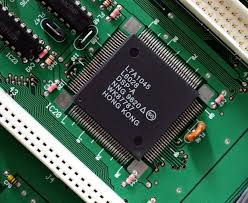
\includegraphics[width=0.9\linewidth]{fig01}
	\caption{Pie de Figura 01}
	\label{fig:01}
\end{figure}
\end{lstlisting}

\begin{figure}[!htb]
	\centering
	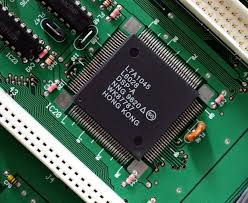
\includegraphics[width=0.9\linewidth]{fig01}
	\caption{Pie de Figura 01}
	\label{fig:01}
\end{figure}

Para que la figura utilice dos columnas 

\begin{lstlisting}[language=bash]
\begin{figure*}[!htb]
	\centering
	
\includegraphics[width=0.9\linewidth]{fig02}
	\caption{Pie de Figura 02}
	\label{Pie de Figura 02}
\end{figure*}
\end{lstlisting}

\begin{figure*}[!htb]
	\centering
	
\includegraphics[width=0.9\linewidth]{fig02}
	\caption{Pie de Figura 02}
	\label{Pie de Figura 02}
\end{figure*}

Para agrupar varias figuras se utiliza el comando 

\begin{lstlisting}[language=bash]
\begin{figure}[!htb]
     \centering
     \begin{subfigure}[b]{0.4\textwidth}
         \centering
         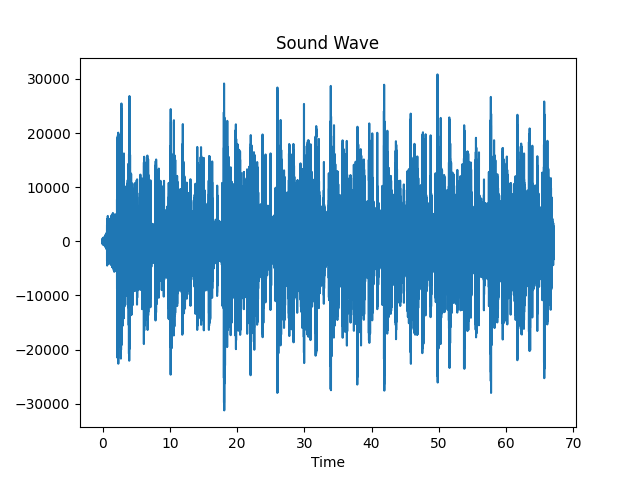
\includegraphics[width=\textwidth]{fig03a}
         \caption{Pie de Figura 03a}
         \label{fig:03a}
     \end{subfigure}
     \hfill
     \begin{subfigure}[b]{0.4\textwidth}
         \centering
         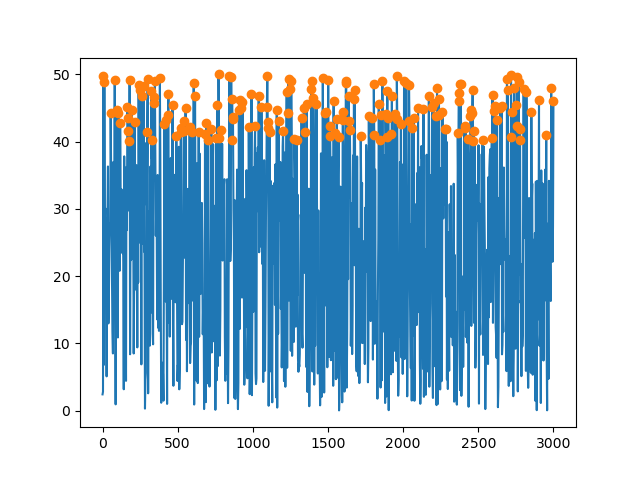
\includegraphics[width=\textwidth]{fig03b}
         \caption{Pie de Figura 03b}
         \label{fig:03b}
     \end{subfigure}
     \hfill
     \begin{subfigure}[b]{0.4\textwidth}
         \centering
         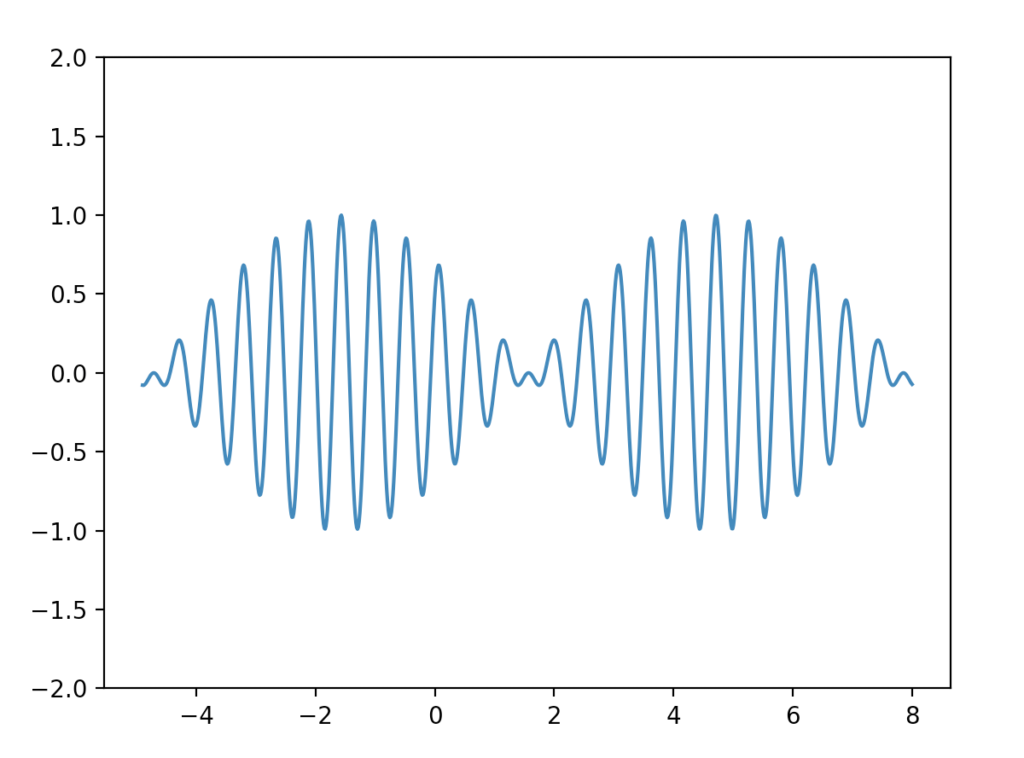
\includegraphics[width=\textwidth]{fig03c}
         \caption{Pie de Figura 03c}
         \label{fig:03c}
     \end{subfigure}
        \caption{Pie de Figura 03}
        \label{fig:03}
\end{figure}
\end{lstlisting}

\begin{figure}[htb!]
    \centering
    \begin{subfigure}[b]{0.4\textwidth}
        \centering
        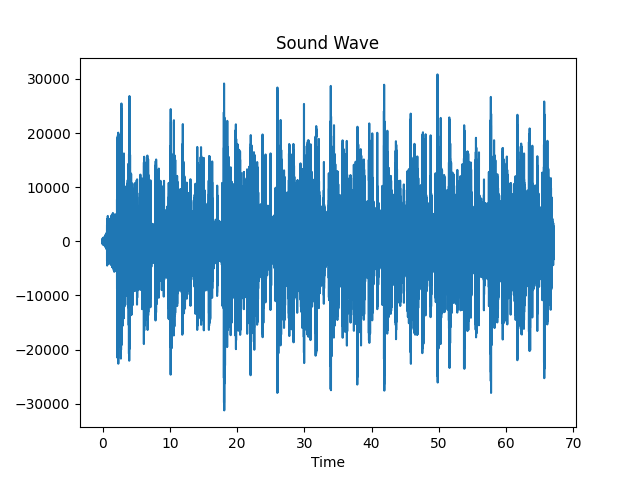
\includegraphics[width=\textwidth]{fig03a}
        \caption{Pie de Figura 03a}
        \label{fig:03a}
    \end{subfigure}
    \hfill
    \begin{subfigure}[b]{0.4\textwidth}
        \centering
        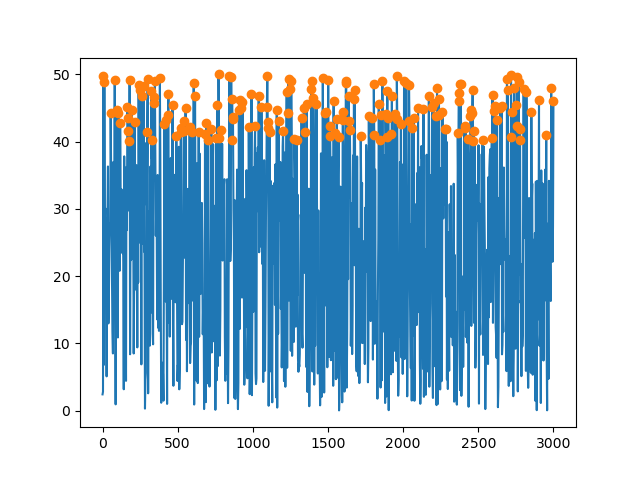
\includegraphics[width=\textwidth]{fig03b}
        \caption{Pie de Figura 03b}
        \label{fig:03b}
    \end{subfigure}
    \hfill
    \begin{subfigure}[b]{0.4\textwidth}
        \centering
        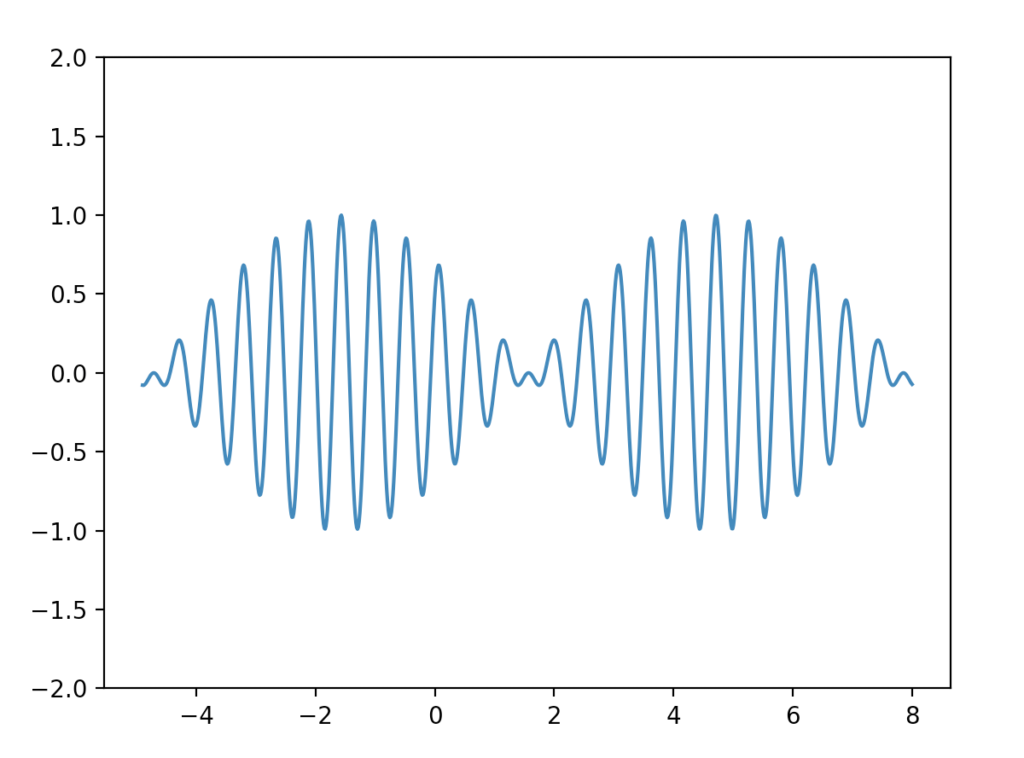
\includegraphics[width=\textwidth]{fig03c}
        \caption{Pie de Figura 03c}
        \label{fig:03c}
    \end{subfigure}
       \caption{Pie de Figura 03}
       \label{fig:03}
\end{figure}

\section{Tablas}

Las tablas se recomiendan cuando se necesita presentar datos de forma estructurada y fácil de comparar, especialmente cuando hay múltiples valores, variables o condiciones experimentales que deben mostrarse de manera clara y concisa. Son particularmente útiles en artículos científicos de ingeniería para mostrar resultados numéricos, parámetros técnicos, especificaciones de componentes, configuraciones experimentales o comparaciones entre métodos.

Se deben colocar lo más cerca posible del texto donde se mencionan o analizan, preferentemente después de la primera referencia a ellas. Cada tabla debe llevar un título descriptivo y numerado, y estar acompañada de una explicación o análisis en el cuerpo del texto. Se recomienda evitar tablas excesivamente grandes o con información redundante, y solo incluir aquellas que aporten valor real a la comprensión del trabajo.

Las tablas se conforman solamente de tres líneas horizontales, ninguna vertical

\begin{lstlisting}[language=bash]
\begin{table}[htb!]
    \centering
    \caption{Titulo de la tabla} 
    \begin{tabular}{cc} 
        \toprule
         Tap   & Coeficiente \\ 
         \midrule
         h[-2]=h[2] & -0.09972695 \\
         h[-1]=h[1] & 0.59466396 \\
        \bottomrule
        \end{tabular}
    \label{tab:01}
\end{table}
\end{lstlisting}

\begin{table}[htb!]
    \centering
    \caption{Título de la tabla} 
    \begin{tabular}{cc} 
        \toprule
         Tap   & Coeficiente \\ 
         \midrule
         h[-2]=h[2] & -0.09972695 \\
         h[-1]=h[1] & 0.59466396 \\
        \bottomrule
        \end{tabular}
    \label{tab:01}
\end{table}

Para tablas que ocupen dos columnas se utiliza el siguiente código:

\begin{lstlisting}[language=bash]
\begin{table*}[htb!]
    \centering
    \caption{Titulo de la tabla}
    \begin{tabular}{ccccccc}
    \toprule
    Parametro & Valor 1 & Valor 2 & Valor 3 & Valor 4 & Valor 5 & Unidad \\
    \midrule
    Resistencia & 100 & 220 & 10 & 47 & 12 & Ohm \\
    Capacitancia & 10 & 47 & 50 & 60 & 12 & $\mu$F \\
    Frecuencia & 50 & 60 & 100 & 220 & 10 & Hz \\
    Tension & 5 & 12 & 10 & 47 & 50 & V \\
    \bottomrule
    \end{tabular}
    \label{tab:02}
\end{table*}
\end{lstlisting}

\begin{table*}[htb!]
    \centering
    \caption{Título de la tabla}
    \begin{tabular}{ccccccc}
    \toprule
    Parámetro & Valor 1 & Valor 2 & Valor 3 & Valor 4 & Valor 5 & Unidad \\
    \midrule
    Resistencia & 100 & 220 & 10 & 47 & 12 &Ohm \\
    Capacitancia & 10 & 47 & 50 & 60 & 12 & $\mu$F \\
    Frecuencia & 50 & 60 & 100 & 220 & 10 & Hz \\
    Tensión & 5 & 12 & 10 & 47 & 50 & V \\
    \bottomrule
    \end{tabular}
    \label{tab:02}
\end{table*}

Para tablas que ocupen dos columnas y que tengan notas al pie, se utiliza el siguiente código:

\begin{lstlisting}
\begin{table*}[htb!]
    \centering
    \begin{threeparttable}
    \small
    \caption{Titulo de la tabla}
    \begin{tabular}{m{3em}m{5em}m{7em}m{7em}m{2em}m{2em}m{2em}m{6em}m{5em}}
        \toprule
         Gas & Principales fuentes & Concentraciones preindustriales & Concentraciones actuales & \multicolumn{3}{m{9em}}{Potenciales de calentamiento global} & Crecimiento (ritmo anual) & Vida atmosferica \\
         & & & & 20 & 100 & 500 & & \\
         \midrule
         Bioxido de carbono $CO_2$* & Quema de combustible fosiles, produccion de cemento, etc. & 280 & 350 & 1 & 1 & 1 & 1.6 & 50*200 \\
         Metano $CH_4$* & Cultivo de arroz, rellenos sanitarios, ganaderia, etc. & 0.8 & 1.7 & 62 & 24.5 & 75 & 0.02 & 10 \\
         Oxido nitroso $ N_20$* & Agricultura (pastoreo en regiones tropicales),  quema de biomasa, etc. & 288 & 310 & 290 & 320 & 180 & 0.8 & 150 \\
         \bottomrule
    \end{tabular}
    \begin{tablenotes}
        \item [*]	Partes por millon
        \item [**]	Partes por mil millones
    \end{tablenotes}
    \end{threeparttable}
    \label{tab:03}
\end{table*}
\end{lstlisting}

\begin{table*}[htb!]
    \centering
    \begin{threeparttable}
    \small
    \caption{Título de la tabla}
    \begin{tabular}{m{3em}m{5em}m{7em}m{7em}m{2em}m{2em}m{2em}m{6em}m{5em}}
        \toprule
         Gas & Principales fuentes & Concentraciones preindustriales & Concentraciones actuales & \multicolumn{3}{m{9em}}{Potenciales de calentamiento global} & Crecimiento (ritmo anual) & Vida atmosférica \\
         & & & & 20 & 100 & 500 & & \\
         \midrule
         Bióxido de carbono $CO_2$* & Quema de combustible fósiles, producción de cemento, etc. & 280 & 350 & 1 & 1 & 1 & 1.6 & 50*200 \\
         Metano $CH_4$* & Cultivo de arroz, rellenos sanitarios, ganadería, etc. & 0.8 & 1.7 & 62 & 24.5 & 75 & 0.02 & 10 \\
         Oxido nitroso $ N_20$* & Agricultura (pastoreo en regiones tropicales),  quema de biomasa, etc. & 288 & 310 & 290 & 320 & 180 & 0.8 & 150 \\
         \bottomrule
    \end{tabular}
    \begin{tablenotes}
        \item [*]	Partes por millón
        \item [**]	Partes por mil millones
    \end{tablenotes}
    \end{threeparttable}
    \label{tab:03}
\end{table*}

\section{Citas y referencias}

La cantidad adecuada de referencias depende del tipo de trabajo, su profundidad y el campo de estudio. Sin embargo, en general para un artículo en el área de ingeniería y tecnología, se recomienda lo siguiente:

\begin{enumerate}
    \item Artículos cortos o técnicos: entre 10 y 20 referencias suelen ser suficientes para sustentar el contexto, justificar la metodología y comparar resultados.
    \item Artículos de investigación completos: entre 20 y 40 referencias es una cantidad razonable para mostrar el dominio del tema, incluir antecedentes relevantes y ubicar el trabajo dentro del estado del arte.
    \item Revisiones bibliográficas o artículos de revisión: pueden contener 50 o más referencias, ya que su objetivo principal es analizar la literatura existente.
\end{enumerate}

Finalmente, las referencias se deben de agregar en el archivo referencias.bib en formato bib. 

\begin{lstlisting}
@article{wyglinski2016revolutionizing,
  title={Revolutionizing software defined radio: case studies in hardware, software, and education},
  author={Wyglinski, Alexander M and Orofino, Don P and Ettus, Matthew N and Rondeau, Thomas W},
  journal={IEEE Communications magazine},
  volume={54},
  number={1},
  pages={68--75},
  year={2016},
  publisher={IEEE}
}
\end{lstlisting}

Las referencias van a ir apareciendo de acuerdo al orden en el que se van citando con el comando.

\begin{lstlisting}[language=bash]
    \cite{wyglinski2016revolutionizing}
\end{lstlisting}

En el texto aparecera \cite{wyglinski2016revolutionizing} y en la bibliografia aparecera el formato de la referencia.
%----------------------------------------------------------------------------------------
%	REFERENCIAS
%----------------------------------------------------------------------------------------

% Las referencias se deben de agregar en el archivo referencias.bib en formato bib. 

\printbibliography

%----------------------------------------------------------------------------------------

\end{document}
